\chapter{कोशिका-कंकाल की गतिकी और कोशिका-गतिशीलता}\label{ch:b3:cytoskeleton-motility}

किसी ऊतक में किसी जीवाणु का पीछा करता कोई उदासीनरागी प्रति मिनट दस
माइक्रोमीटर रेंगता है और गंध बदलते ही सेकंडों में दिशा बदल देता है।
किसी चालक न्यूरॉन की कोशिका-काय में बनी तंत्रिका-संचारक की कोई पुटिका
तंत्रिकाक्ष से होकर एक मीटर नीचे पैर तक जाती है, किसी ऐसे मोटर प्रोटीन
से खिंचती हुई जो आठ-नैनोमीटर के डग भरता है, प्रति सेकंड सौ, पूरे पखवाड़े
तक। श्वासनली की भीतरी परत के \omterm{def:b3:cytoskeleton-motility:cilia}{पक्ष्माभ} प्रति सेकंड बारह बार समन्वित
लहरों में हिलते हैं और दिन भर की साँस में आई धूल गले तक ऊपर पहुँचा देते
हैं। यह सब तीन प्रकार के प्रोटीन तंतु करते हैं जो सेकंडों में जुड़ते और
टूटते हैं, और वे मोटर करते हैं जो प्रति डग ATP का एक अणु जलाते हैं।
कोशिका-कंकाल किसी स्थिर ढाँचे के अर्थ में कंकाल है ही नहीं; वह लगातार
आवागमन में रहने वाले बहुलकों का समुच्चय है, जिनकी गतिकी \emph{ही} आकार,
विभाजन और गति की क्रियाविधि है। यह अध्याय बहुलकों और उनकी बलगतिकी,
मोटरों और उन्हें सीमित करती भौतिकी, कोशिका के रेंगने, और \omterm{def:b3:cytoskeleton-motility:cilia}{पक्ष्माभों} तथा
कशाभों के हिलने को लेता है।

\section{तीन बहुलक}

\begin{definition}[ऐक्टिन तंतु, सूक्ष्मनलिकाएँ, मध्यवर्ती तंतु]\label{def:b3:cytoskeleton-motility:filaments}
\index{ऐक्टिन तंतु}\index{सूक्ष्मनलिका}\index{मध्यवर्ती तंतु}\index{ध्रुवता!तंतुओं की}\index{तारककाय}
कोई \emph{ऐक्टिन तंतु} गोलिकाकार ऐक्टिन का दो-लड़ी कुंडलित बहुलक है,
\qty{7}{nm} मोटा, जिसकी हर उपइकाई अक्ष के साथ \qty{2.7}{nm} की है, और
जो ध्रुवीय है: \emph{काँटेदार} (धन) सिरा \emph{नुकीले}
(ऋण) सिरे से तेज़ी से बढ़ता है, और हर उपइकाई कोई ATP ढोती है जिसका
जुड़ने के बाद जल-अपघटन हो जाता है। कोई \emph{सूक्ष्मनलिका} \qty{25}{nm}
बाह्य व्यास की खोखली नली है, जो $\alpha\beta$-ट्यूबुलिन द्विलकों के
तेरह आद्यतंतुओं से बनी है (प्रति द्विलक \qty{8}{nm}), और वह भी ध्रुवीय
है, जिसका \emph{धन} सिरा तेज़ी से बढ़ता है और \emph{ऋण} सिरा प्रायः
केंद्रक के पास \emph{तारककाय} पर लंगर डाले रहता है; $\beta$ उपइकाई
जुड़ने के बाद अपना GTP जल-अपघटित करती है। कोई \emph{मध्यवर्ती तंतु}
\qty{10}{nm} का ऐसा रस्सा है जो कुंडलित-कुंडली प्रोटीनों से बना है
(उपकला में केराटिन, मध्यजनोतक में वाइमेंटिन, तंत्रिकाक्षों में
न्यूरोतंतु, केंद्रक-आवरण के नीचे लैमिन), अध्रुवीय, बिना किसी
न्यूक्लियोटाइड के, और कहीं अधिक स्थिर --- किसी गतिक पटरी के बजाय तनाव
ढोने वाला कोई तार। ऐक्टिन अधिकतर जीवद्रव्य-कला के नीचे और उभारों में
बैठता है; सूक्ष्मनलिकाएँ तारककाय से विकीर्ण होती हैं और दूर तक परिवहन
की पटरियों तथा तर्कु का काम करती हैं; मध्यवर्ती तंतु कोशिका और उसके
केंद्रक को यांत्रिक दृढ़ता देते हैं।
\end{definition}

\begin{omfigure}
\begin{tikzpicture}[every node/.style={font=\scriptsize}, >=stealth]
  % actin
  \begin{scope}
    \foreach \i in {0,...,11} { \fill[omThm!70] ({\i*0.4},{0.12*sin(\i*60)}) circle (0.17); }
    \node[below, align=center] at (2.2,-0.5) {ऐक्टिन तंतु, \qty{7}{nm}\\दो-लड़ी कुंडली, ATP-ऐक्टिन\\उपइकाई अक्ष के साथ \qty{2.7}{nm}};
    \node[left] at (-0.3,0) {$-$ नुकीला}; \node[right] at (4.6,0) {काँटेदार $+$};
  \end{scope}
  % microtubule
  \begin{scope}[xshift=7.2cm]
    \draw[thick, fill=omDef!25] (0,-0.55) rectangle (4.4,0.55);
    \foreach \y in {-0.35,-0.15,0.05,0.25} \draw[omDef] (0,\y) -- (4.4,\y);
    \foreach \x in {0.4,0.8,...,4.0} \draw[omDef] (\x,-0.55) -- (\x,0.55);
    \draw[thick] (4.4,0) ellipse (0.18 and 0.55); \draw[thick, fill=white] (4.4,0) ellipse (0.09 and 0.38);
    \node[below, align=center] at (2.2,-0.65) {सूक्ष्मनलिका, \qty{25}{nm}\\$\alpha\beta$-ट्यूबुलिन (GTP) के 13 आद्यतंतु\\द्विलक \qty{8}{nm} लंबा};
    \node[left] at (-0.2,0) {$-$}; \node[right] at (4.7,0) {$+$};
  \end{scope}
  % intermediate filament
  \begin{scope}[yshift=-2.9cm, xshift=3.6cm]
    \foreach \dd in {-0.12,0,0.12} \draw[omMeth!70!black, thick] plot[domain=0:4.4, samples=60] (\x, {\dd + 0.1*sin(\x*200 + \dd*400)});
    \node[below, align=center] at (2.2,-0.4) {मध्यवर्ती तंतु, \qty{10}{nm}\\कुंडलित-कुंडली रस्सा (केराटिन, वाइमेंटिन, लैमिन), कोई ध्रुवता नहीं, कोई न्यूक्लियोटाइड नहीं};
  \end{scope}
\end{tikzpicture}

{\small तीनों तंतु व्यास के अनुपात में। ऐक्टिन और ट्यूबुलिन के बहुलक
ध्रुवीय हैं और जुड़ने के बाद किसी न्यूक्लियोटाइड का जल-अपघटन करते हैं,
और यही उन्हें गतिक बनाता है; \omterm{def:b3:cytoskeleton-motility:filaments}{मध्यवर्ती तंतु} सहनशीलता के लिए बना कोई
अध्रुवीय रस्सा है।}
\end{omfigure}

\begin{omfigure}
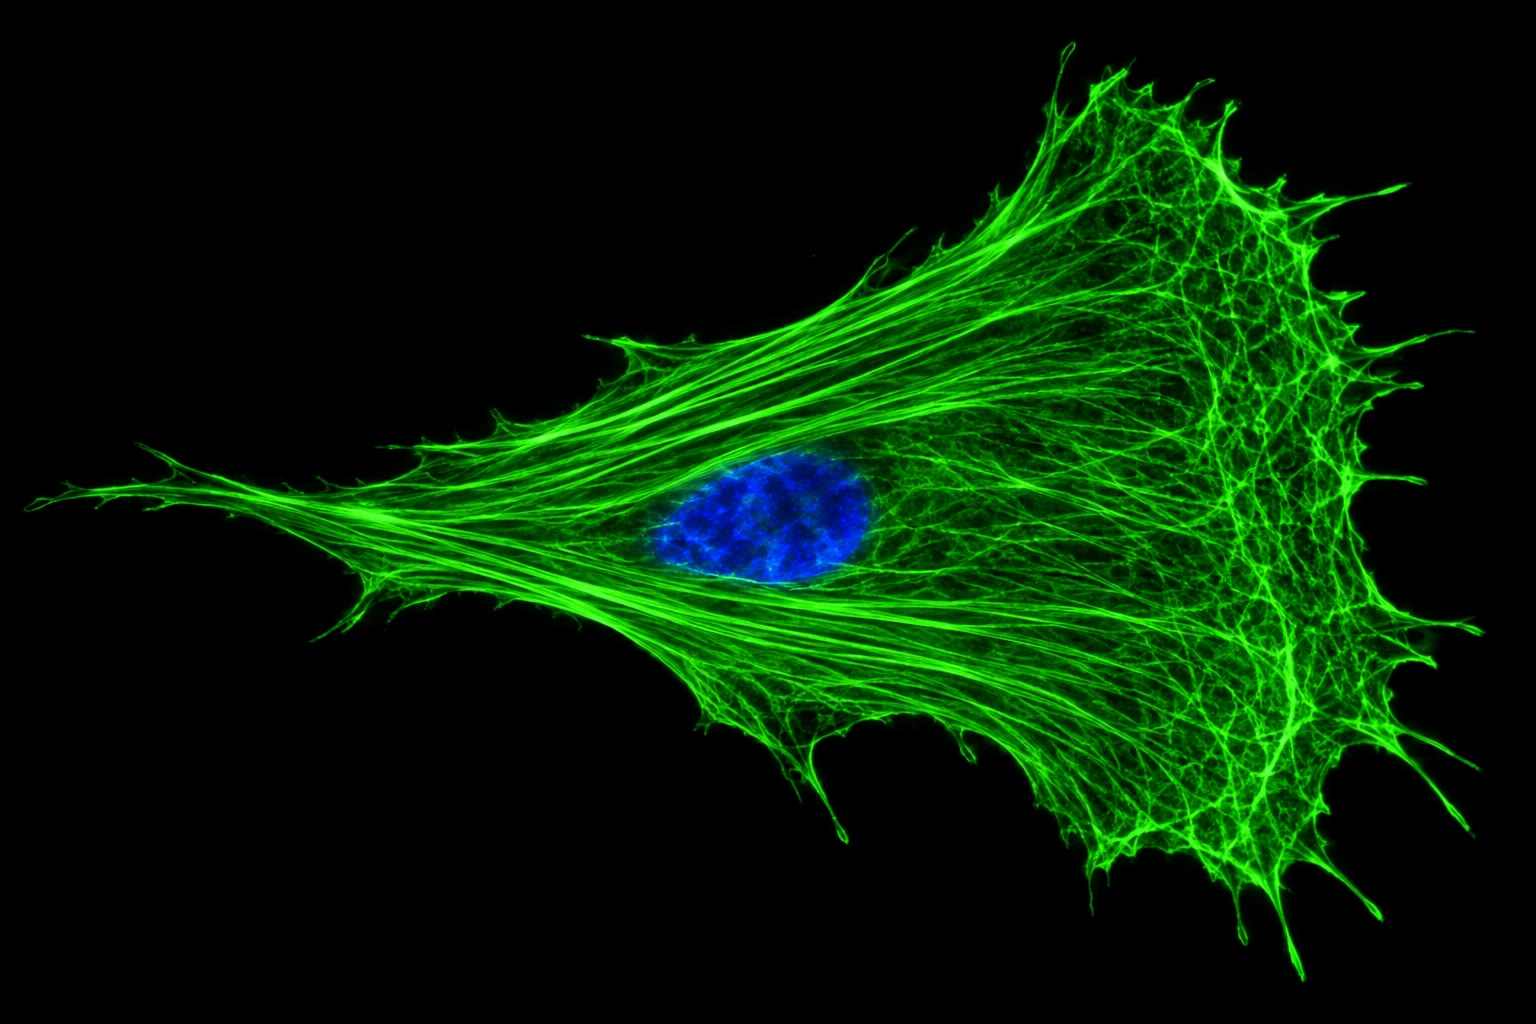
\includegraphics[width=0.54\linewidth]{images/book5/ai/b5-09-fibroblast-actin.jpg}\hspace{0.03\linewidth}
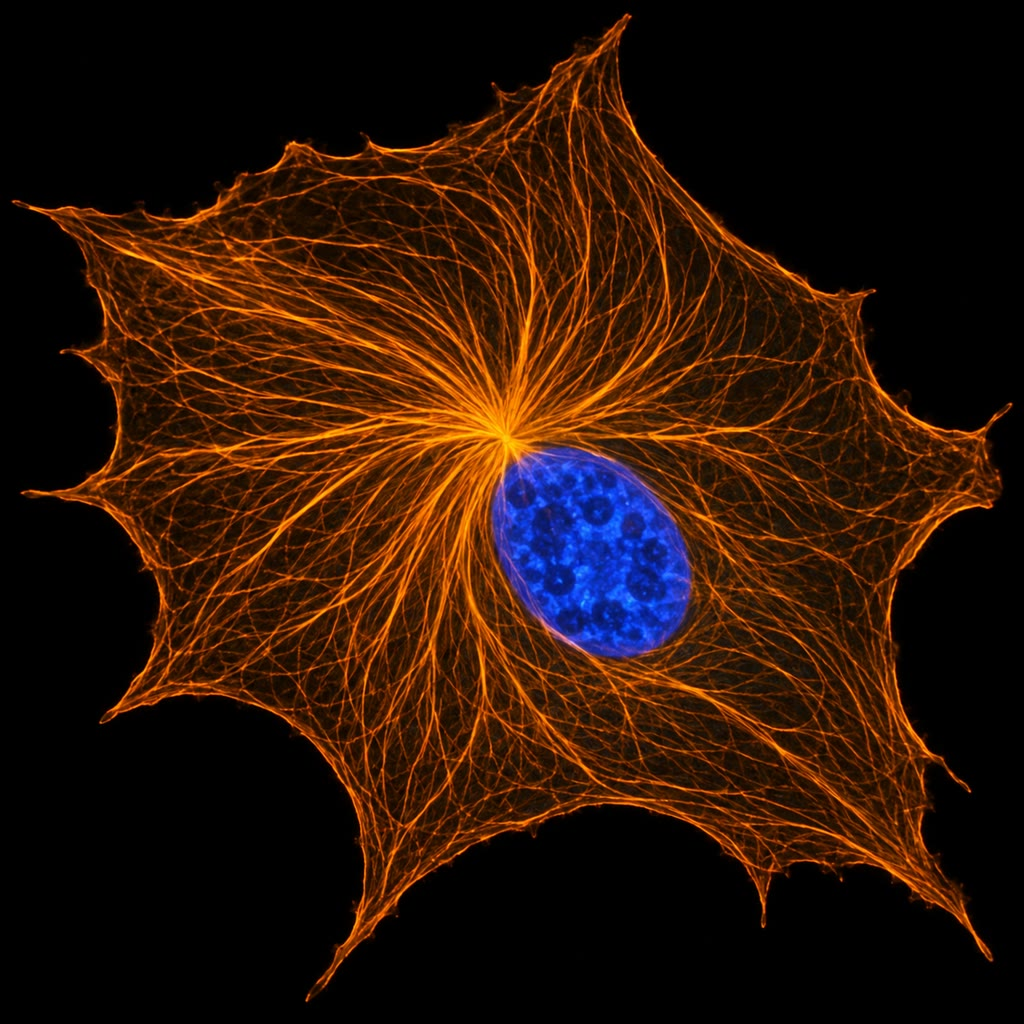
\includegraphics[width=0.36\linewidth]{images/book5/ai/b5-09-microtubules.jpg}

{\small बाएँ: किसी प्रवसन करते तंतुकोरक में ऐक्टिन (हरा) --- काय के
आर-पार प्रतिबल-तंतु, और दाईं ओर चौड़े अग्रणी किनारे पर सघन जाल। दाएँ:
केंद्रक (नीला) के बगल के \omterm{def:b3:cytoskeleton-motility:filaments}{तारककाय} से कोशिका-किनारे तक विकीर्ण होती
\omterm{def:b3:cytoskeleton-motility:filaments}{सूक्ष्मनलिकाएँ} (नारंगी)।}
\end{omfigure}

\section{किसी बहुलक की बलगतिकी}

\begin{theorem}[क्रांतिक सांद्रता और चक्रचालन]\label{thm:b3:cytoskeleton-motility:treadmilling}
\index{क्रांतिक सांद्रता}\index{चक्रचालन}
मान लीजिए किसी तंतु का कोई सिरा दर $k_{\text{जुड़}}C$ से उपइकाइयाँ जोड़ता
है, जहाँ $C$ मुक्त एकलक सांद्रता है, और उन्हें दर
$k_{\text{छूट}}$ से खोता है। सिरा तब बढ़ता है जब $C$ उसकी \emph{\omterm{thm:b3:cytoskeleton-motility:treadmilling}{क्रांतिक
सांद्रता}} $C_{c} = k_{\text{छूट}}/k_{\text{जुड़}}$ से ऊपर हो और उससे नीचे
सिकुड़ता है। यदि दोनों सिरों की \omterm{thm:b3:cytoskeleton-motility:treadmilling}{क्रांतिक सांद्रताएँ} भिन्न हों, $C_{c}^{+}
< C_{c}^{-}$, तो उस स्थायी अवस्था पर जहाँ तंतु न लंबा होता है न छोटा,
एकलक सांद्रता होती है
\[
C_{\text{स्था}} = \frac{k_{\text{छूट}}^{+} + k_{\text{छूट}}^{-}}
{k_{\text{जुड़}}^{+} + k_{\text{जुड़}}^{-}},
\qquad C_{c}^{+} < C_{\text{स्था}} < C_{c}^{-},
\]
और धन सिरा बढ़ता है जबकि ऋण सिरा उसी दर
$J = k_{\text{जुड़}}^{+}C_{\text{स्था}} - k_{\text{छूट}}^{+} > 0$ से
सिकुड़ता है: उपइकाइयाँ तंतु से होकर धन से ऋण की ओर बहती हैं ---
\emph{चक्रचालन} --- और इसकी कीमत प्रति उपइकाई एक न्यूक्लियोटाइड का
जल-अपघटन है।
\end{theorem}
\begin{proof}
किसी सिरे पर शुद्ध दर $k_{\text{जुड़}}C - k_{\text{छूट}}$ है, जो
$C_{c}$ पर शून्य है। अचर लंबाई के लिए दोनों शुद्ध दरों का योग शून्य
होना चाहिए, जिससे $C_{\text{स्था}}$ मिलता है; वह दोनों \omterm{thm:b3:cytoskeleton-motility:treadmilling}{क्रांतिक
सांद्रताओं} के बीच पड़ता है क्योंकि वह उनका भारित माध्य है ($C_{\text{स्था}} =
(k_{\text{जुड़}}^{+}C_{c}^{+} + k_{\text{जुड़}}^{-}C_{c}^{-})/(k_{\text{जुड़}}^{+}
+ k_{\text{जुड़}}^{-})$)। $C_{c}^{+}$ से ऊपर धन सिरा बढ़ता है;
$C_{c}^{-}$ से नीचे ऋण सिरा सिकुड़ता है; अभिवाह धन सिरे की शुद्ध दर है।
एक ही रासायनिक बहुलक के दोनों सिरों का $C_{c}$ एक ही होता (वही
साम्य नियतांक), इसलिए किसी अंतर के लिए ज़रूरी है कि उपइकाई जुड़ने के बाद
बदले --- ATP या GTP का जल-अपघटन --- जो सिरों को भिन्न बनाता है और बहाव
की कीमत चुकाता है।
\end{proof}

\begin{example}[परखनली में ऐक्टिन]\label{ex:b3:cytoskeleton-motility:actin-numbers}
ऐक्टिन-ATP के लिए $k_{\text{जुड़}}^{+} = \qty{11.6}{\micro M^{-1}.s^{-1}}$,
$k_{\text{छूट}}^{+} = \qty{1.4}{s^{-1}}$ ($C_{c}^{+} = \qty{0.12}{\micro
M}$); $k_{\text{जुड़}}^{-} = \qty{1.3}{\micro M^{-1}.s^{-1}}$,
$k_{\text{छूट}}^{-} = \qty{0.8}{s^{-1}}$ ($C_{c}^{-} = \qty{0.6}{\micro
M}$)। तब $C_{\text{स्था}} = 2.2/12.9 = \qty{0.17}{\micro M}$ और $J =
11.6\times 0.17 - 1.4 = 0.6$ उपइकाई प्रति सेकंड: \qty{1.6}{nm/s},
अगोचर। किसी कोशिका में तंतु सौ गुना तेज़ी से चक्रचालन करते हैं, क्योंकि
कोफ़िलिन नुकीले सिरों से पुराना ADP-ऐक्टिन काटकर छील देता है, प्रोफ़िलिन
काँटेदार सिरों पर ताज़ा ATP-ऐक्टिन चढ़ाता है, और टोपी-प्रोटीन तय करते
हैं कि कौन-से काँटेदार सिरे बढ़ भी सकते हैं: नंगा बहुलक क्रियाविधि देता
है, नियामक गति देते हैं।
\end{example}

\begin{omfigure}
\begin{tikzpicture}
\begin{axis}[
  width=0.7\linewidth, height=5.6cm,
  axis x line=bottom, axis y line=left,
  xmin=0, xmax=1.0, ymin=-1.6, ymax=4,
  xlabel={मुक्त ऐक्टिन ($\unit{\micro M}$)}, ylabel={शुद्ध दर (उपइकाई/s)},
  xlabel style={font=\small, at={(axis description cs:0.5,-0.12)}, anchor=north},
  ylabel style={font=\small},
  tick label style={font=\small}, xtick={0,0.2,0.4,0.6,0.8,1.0}, ytick={-1,0,1,2,3,4},
  clip=false,
]
\addplot[thin, gray, domain=0:1.0, samples=2] {0};
\addplot[very thick, omThm, domain=0:0.46, samples=2] {11.6*x-1.4};
\addplot[very thick, omDef, domain=0:1.0, samples=2] {1.3*x-0.8};
\draw[dashed, gray] (axis cs:0.17,-1.6) -- (axis cs:0.17,4);
\node[font=\scriptsize, omThm, anchor=south east] at (axis cs:0.44,3.1) {काँटेदार सिरा};
\node[font=\scriptsize, omDef, anchor=north west] at (axis cs:0.62,-0.25) {नुकीला सिरा};
\node[font=\scriptsize, anchor=south west] at (axis cs:0.19,3.5) {$C_{\text{स्था}}$};
\fill[omThm] (axis cs:0.12,0) circle (2pt); \node[font=\scriptsize, anchor=north east] at (axis cs:0.11,-0.05) {$C_{c}^{+}$};
\fill[omDef] (axis cs:0.6,0) circle (2pt); \node[font=\scriptsize, anchor=south west] at (axis cs:0.61,0.05) {$C_{c}^{-}$};
\end{axis}
\end{tikzpicture}

{\small उदाहरण के दर-नियतांकों के साथ, मुक्त एकलक के सामने किसी \omterm{def:b3:cytoskeleton-motility:filaments}{ऐक्टिन
तंतु} के हर सिरे की शुद्ध वृद्धि-दर। दोनों \omterm{thm:b3:cytoskeleton-motility:treadmilling}{क्रांतिक सांद्रताओं} के बीच
काँटेदार सिरा बढ़ता है और नुकीला सिरा सिकुड़ता है; बिंदुदार रेखा पर
दोनों ठीक-ठीक कट जाते हैं और तंतु चक्रचालन करता है।}
\end{omfigure}

\begin{definition}[गतिक अस्थिरता]\label{def:b3:cytoskeleton-motility:instability}
\index{गतिक अस्थिरता}\index{GTP टोपी}\index{विपर्यय}
\omterm{def:b3:cytoskeleton-motility:filaments}{सूक्ष्मनलिकाएँ} चक्रचालन से भी विचित्र कुछ करती हैं। कोई बढ़ता धन
सिरा ताज़ा जुड़े द्विलकों की कोई \emph{GTP टोपी} ढोता है; उसके पीछे GTP
का जल-अपघटन हो जाता है, और GDP-ट्यूबुलिन, जो मुड़ी संरूपता पसंद करता है,
जालक में तनाव के नीचे सीधा थामे रखा जाता है। यदि टोपी खो जाए --- सिरा
रुक जाए, या वृद्धि धीमी पड़े --- तो तने हुए आद्यतंतु बाहर की ओर छिल जाते
हैं और \omterm{def:b3:cytoskeleton-motility:filaments}{सूक्ष्मनलिका} \qty{300}{nm/s} से छोटी होती है, यानी अपनी
वृद्धि-दर से बीस गुना: यही कोई \emph{विपर्यय} है, जो तब समाप्त होता है
जब कोई GTP द्विलक आ बैठे और नई टोपी बन जाए (कोई \emph{उद्धार})। इसलिए
किसी एक समष्टि में कुछ \omterm{def:b3:cytoskeleton-motility:filaments}{सूक्ष्मनलिकाएँ} बढ़ती हैं जबकि पड़ोसिनें ढह जाती
हैं: यही \emph{गतिक अस्थिरता} है। इससे कोई कोशिका हर कुछ मिनट में धन
सिरों से अपने ही आयतन की टोह ले सकती है और \omterm{def:b3:cytoskeleton-motility:filaments}{तारककाय} के हिलने या कोशिका
के विभाजित होने पर पूरी सज्जा फिर बना सकती है। कोशिका उसे ऐसे प्रोटीनों
से साधती है जो धन सिरों का पीछा करते हैं, \omterm{def:b3:cytoskeleton-motility:filaments}{सूक्ष्मनलिकाओं} को स्थिर करते
(टाउ, MAP2), काटते (कैटानिन) या विबहुलकित (काइनेसिन-13) करते हैं;
औषधें कोल्चिसीन और विंका क्षाराभ जुड़ाई रोकती हैं और टैक्सॉल टूटन
रोकता है, और ये सब समसूत्री तर्कु के विष हैं जो कर्कट के विरुद्ध काम
में लिए जाते हैं।
\end{definition}

\begin{proof}[प्रमाण-सामग्री]
मिचिसन और किर्शनर (1984) ने पात्रे \omterm{def:b3:cytoskeleton-motility:filaments}{तारककायों} से उगाई गई
\omterm{def:b3:cytoskeleton-motility:filaments}{सूक्ष्मनलिकाओं} की समष्टियाँ देखीं। ट्यूबुलिन को \omterm{thm:b3:cytoskeleton-motility:treadmilling}{क्रांतिक सांद्रता} से
नीचे तनु करने पर उन्हें आशा थी कि सारी \omterm{def:b3:cytoskeleton-motility:filaments}{सूक्ष्मनलिकाएँ} धीरे-धीरे छोटी
होंगी; इसके बजाय \omterm{def:b3:cytoskeleton-motility:filaments}{सूक्ष्मनलिकाओं} की संख्या गिरी जबकि बचे हुए बढ़ते रहे
--- कुछ पूरी तरह और तेज़ी से टूट चुके थे, कुछ बिलकुल नहीं। बाद में
वीडियो सूक्ष्मदर्शिकी से फ़िल्माई गई अलग-अलग \omterm{def:b3:cytoskeleton-motility:filaments}{सूक्ष्मनलिकाएँ} अचानक
स्थिर वृद्धि और तीव्र संकुचन की प्रावस्थाओं के बीच बदलती दिखीं।
\omterm{def:b3:cytoskeleton-motility:instability}{GTP टोपी} ने दोनों समझाए: केवल टोपी वाले सिरे बढ़ते हैं, और टोपी का
खोना कोई दुर्लभ, सब-या-कुछ-नहीं घटना है।
\end{proof}

\section{मोटर}

\begin{definition}[मोटर प्रोटीन]\label{def:b3:cytoskeleton-motility:motors}
\index{मायोसिन}\index{काइनेसिन}\index{डाइनीन}\index{अनुवर्तिता}
कोई \emph{मोटर प्रोटीन} ATP जल-अपघटन की मुक्त ऊर्जा को किसी तंतु के
साथ-साथ निर्देशित गति में बदलता है: ऐक्टिन पर \emph{मायोसिन} (मायोसिन
II, पेशी और संकुचन की मोटर, काँटेदार सिरे की ओर; मायोसिन V, \qty{36}{nm}
डग भरता दो-सिर वाला पुटिका-वाहक), \omterm{def:b3:cytoskeleton-motility:filaments}{सूक्ष्मनलिकाओं} पर धन सिरे की ओर
\emph{काइनेसिन} (काइनेसिन-1 प्रति ATP \qty{8}{nm}, यानी एक ट्यूबुलिन
द्विलक, हाथ-दर-हाथ, लगभग \qty{800}{nm/s} पर), और ऋण सिरे की ओर
\emph{डाइनीन} (कोशिकाद्रव्यी डाइनीन, अपने संयोजक डाइनैक्टिन के साथ, भार
वापस कोशिका-केंद्र तक खींचती है; \omterm{def:b3:cytoskeleton-motility:cilia}{अक्षसूत्री डाइनीन} \omterm{def:b3:cytoskeleton-motility:cilia}{पक्ष्माभ} मोड़ती
हैं)। कोई मोटर \emph{अनुवर्ती} है यदि वह छूटने से पहले अनेक डग भरे:
काइनेसिन-1 अकेले लगभग एक माइक्रोमीटर, यानी सौ डग, चलती है;
मायोसिन II का एक अकेला सिर एक ही आघात करके छोड़ देता है, इसलिए पेशी को
एक ही तंतु पर सैकड़ों सिर चाहिए। मोटर पटरी की ध्रुवता पढ़ते हैं, इसलिए
किसी कोशिका का भूगोल --- परिधि पर धन सिरे, केंद्र पर ऋण सिरे --- इसका
मानचित्र है कि हर मोटर अपना भार कहाँ ले जाएगी।
\end{definition}

\begin{proof}[प्रमाण-सामग्री]
वेल, रीस और शीत्स (1985) ने \omterm{def:b3:cytoskeleton-motility:motors}{काइनेसिन} को व्हिड्डी के तंत्रिकाक्ष-द्रव्य
के उस प्रोटीन के रूप में पाया जो लेटेक्स मणिकाओं को \omterm{def:b3:cytoskeleton-motility:filaments}{सूक्ष्मनलिकाओं} पर
धन दिशा में सरकाता था, और अगले वर्षों में दो-सिर वाली संरचना, हर कुल की
दिशा और प्रतिगामी साथी \omterm{def:b3:cytoskeleton-motility:motors}{डाइनीन} सुलझा लिए गए। स्वोबोदा, श्मिट, श्नाप और
ब्लॉक (1993) ने किसी एक \omterm{def:b3:cytoskeleton-motility:motors}{काइनेसिन} को ढोती मणिका को किसी प्रकाशिक फंदे
में थामा और उसकी स्थिति नैनोमीटर विभेदन से अंकित की: मणिका
\qty{8}{nm} के असतत डगों में आगे बढ़ी, कम ATP सांद्रता पर प्रति ATP एक,
और लगभग \qty{6}{pN} के बल के सामने ठहर गई। आणविक सीढ़ी सीधे देख ली गई।
\end{proof}

\begin{omfigure}
\begin{tikzpicture}[every node/.style={font=\scriptsize}, >=stealth]
  % left: kinesin on a microtubule
  \begin{scope}
    \draw[thick, fill=omDef!25] (0,0) rectangle (5.4,0.5);
    \foreach \x in {0.4,0.8,...,5.2} \draw[omDef] (\x,0) -- (\x,0.5);
    \node[left] at (-0.1,0.25) {$-$}; \node[right] at (5.5,0.25) {$+$};
    % two heads, stalk, cargo
    \fill[omProp] (2.4,0.72) circle (0.2); \fill[omProp!60] (3.2,0.72) circle (0.2);
    \draw[thick, omProp!80!black] (2.6,0.85) -- (2.85,1.4) -- (3.05,0.85); \draw[thick, omProp!80!black] (2.85,1.4) -- (2.85,2.3);
    \draw[thick, fill=omExo!40] (2.85,2.7) circle (0.4); \node at (2.85,2.7) {भार};
    \draw[->, thick, omThm] (3.4,0.72) arc[start angle=180, end angle=0, radius=0.4] ; \node[right, omThm] at (3.85,1.15) {प्रति ATP \qty{8}{nm}};
    \node[below, align=center] at (2.7,-0.1) {काइनेसिन-1 धन सिरे की ओर हाथ-दर-हाथ चलती है;\\प्रति सेकंड लगभग $100$ डग, \qty{0.8}{\micro m/s}};
  \end{scope}
  % right: optical trap staircase
  \begin{scope}[xshift=7.2cm, yshift=-0.6cm]
  \begin{axis}[
    width=5.6cm, height=4.4cm, axis lines=left,
    xmin=0, xmax=1.0, ymin=0, ymax=40,
    xlabel={समय (s)}, ylabel={स्थिति (nm)},
    xlabel style={font=\scriptsize, at={(axis description cs:0.5,-0.12)}, anchor=north},
    ylabel style={font=\scriptsize},
    tick label style={font=\scriptsize}, xtick={0,0.5,1.0}, ytick={0,8,16,24,32},
  ]
  \addplot[very thick, omProp!80!black, const plot] coordinates {(0,0) (0.18,8) (0.31,16) (0.55,24) (0.71,32) (1.0,32)};
  \end{axis}
  \node[font=\scriptsize, align=center] at (2.8,3.6) {प्रकाशिक फंदे में एक अकेली मोटर,\\कम ATP: \qty{8}{nm} के डग};
  \end{scope}
\end{tikzpicture}

{\small \omterm{def:b3:cytoskeleton-motility:motors}{काइनेसिन} अपनी पटरी पर और प्रकाशिक फंदे में उसका पदचिह्न। दोनों
सिर बारी-बारी चलते हैं, और हर डग मोटर को एक ट्यूबुलिन द्विलक,
\qty{8}{nm}, आगे बढ़ा देता है; कम ATP पर डगों के बीच अगले
न्यूक्लियोटाइड की प्रतीक्षा रहती है और सीढ़ी सीधे दिख जाती है।}
\end{omfigure}

\begin{proposition}[भौतिकी किसी मोटर को क्या देती है]\label{prop:b3:cytoskeleton-motility:physics}
\index{ठहराव बल}\index{तापीय ऊर्जा}\index{विसरण बनाम परिवहन}
कोशिका में एक ATP का जल-अपघटन लगभग \qty{50}{kJ/mol} मुक्त करता है,
यानी प्रति अणु $8\times 10^{-20}$ J। जो मोटर प्रति ATP $d$ आगे बढ़ती है
और बल $F$ के विरुद्ध काम $Fd$ करती है, उसका \emph{\omterm{prop:b3:cytoskeleton-motility:physics}{ठहराव बल}}
$F_{\max} = \Delta G/d$ से अधिक नहीं हो सकता: \omterm{def:b3:cytoskeleton-motility:motors}{काइनेसिन} के \qty{8}{nm}
डग के लिए \qty{10}{pN}; मापा गया \qty{6}{pN} लगभग \qty{60}{\%} की
दक्षता बताता है, जो किसी भी इंजन से अधिक है। \omterm{prop:b3:cytoskeleton-motility:physics}{तापीय ऊर्जा} $k_{B}T =
4.1\times 10^{-21}$ J, यानी \qty{4.1}{pN.nm}, ATP की ऊर्जा का बीसवाँ भाग
ही है पर वह मोटर को ब्राउनी ठोकरों के रूप में लगातार मिलती रहती है;
मोटर ऐसी युक्ति है जो उन्हें एकदिश कर देती है, सिर को आगे विसरित होने
देकर और उतरते ही बाँध लेकर, जिससे रासायनिक ऊर्जा धकेलने पर नहीं, डग को
अनुत्क्रमणीय बनाने पर खर्च होती है। किसी बड़ी कोशिका में मायने रखने
वाली हर दूरी पर मोटर से परिवहन विसरण को हरा देता है: विसरण गुणांक
$D = \qty{1}{\micro
m^2/s}$ वाली किसी पुटिका को समय $L^{2}/2D$ लगता है ताकि वह दूरी $L$ भटके
--- एक माइक्रोमीटर के लिए आधा सेकंड, पर किसी तंत्रिकाक्ष के एक मीटर के
लिए \num{16000} वर्ष --- जबकि \qty{1}{\micro m/s} वाली कोई मोटर वह मीटर
बारह दिन में तय कर लेती है।
\end{proposition}
\admitted

\section{कोई कोशिका कैसे रेंगती है}

\begin{definition}[कोशिका प्रवसन]\label{def:b3:cytoskeleton-motility:migration}
\index{पर्णपाद}\index{Arp2/3 संकुल}\index{केंद्री आसंजन}\index{इंटीग्रिन}\index{Rho GTPase}
कोई रेंगती कोशिका चार चरणों का चक्र दोहराती है। \emph{उभार}: अग्रणी
किनारे पर ऐक्टिन झिल्ली के विरुद्ध किसी चादर में बहुलकित होता है, यानी
\emph{पर्णपाद}, जिसका शाखित जाल \emph{Arp2/3 संकुल} बनाता है, जो किसी
पहले से मौजूद तंतु के पार्श्व से \qty{70}{\degree} पर कोई नया तंतु
आरंभ करता है, जबकि टोपी-प्रोटीन हर तंतु की वृद्धि सीमित करता है और
कोफ़िलिन कुछ माइक्रोमीटर पीछे जाल पुनर्चक्रित कर देता है; गुच्छित
तंतुओं के उँगली जैसे \emph{तंतुपाद} आगे टोह लेते हैं।
\emph{आसंजन}: नया उभार आधार से \emph{इंटीग्रिनों} के ज़रिए जुड़ता है,
जो ऐसे झिल्ली-पारी ग्राही हैं जो बाहर आधात्री प्रोटीनों से और, संयोजक
प्रोटीनों के ज़रिए, भीतर ऐक्टिन से बँधते हैं और \emph{केंद्री आसंजनों}
में गुच्छित रहते हैं। \emph{संकुचन}: \omterm{def:b3:cytoskeleton-motility:motors}{मायोसिन} II आसंजनों पर लंगर डाले
प्रतिबल-तंतुओं को खींचता है और कोशिका-काय को आगे घसीटता है।
\emph{प्रत्याकर्षण}: पीछे के आसंजन छूट जाते हैं और पूँछ भीतर खींच ली
जाती है। इस चक्र का समन्वय \emph{Rho} कुल की तीन \omterm{def:b3:membrane-traffic:coats}{लघु GTPase} करती हैं
--- Rac पर्णपाद चलाती है, Cdc42 तंतुपाद, Rho प्रतिबल-तंतु और संकुचन ---
और वे ही उन ग्राहियों के लक्ष्य हैं जो किसी रासायनिक प्रवणता की दिशा
(रसायनानुचलन) या आधार की कठोरता तथा प्रतिरूप पढ़ते हैं।
\end{definition}

\begin{omfigure}
\begin{tikzpicture}[every node/.style={font=\scriptsize}, >=stealth]
  % substrate
  \draw[very thick, gray] (0,0) -- (12,0); \node[below right, gray] at (0,-0.05) {आधार (आधात्री)};
  % cell outline
  \draw[thick, omDef, fill=omDef!10] (1.0,0.05) .. controls (1.2,1.4) and (3.0,2.3) .. (5.0,2.2) .. controls (7.0,2.1) and (8.6,1.4) .. (9.8,0.6) .. controls (10.3,0.4) and (10.8,0.2) .. (11.2,0.05) -- cycle;
  % nucleus
  \draw[thick, fill=omDef!40] (4.6,1.1) ellipse (1.0 and 0.6); \node at (4.6,1.1) {केंद्रक};
  % lamellipodium: branched actin
  \foreach \p/\a in {(9.9,0.3)/20,(10.1,0.5)/-10,(10.3,0.25)/35,(10.6,0.45)/5,(10.4,0.7)/-25,(9.7,0.7)/15} { \draw[omThm, thick] \p -- ++(\a:0.55); \draw[omThm, thick] \p ++(\a:0.3) -- ++(\a+70:0.35); }
  \node[right, align=left, omThm] at (11.3,1.3) {1. उभार:\\Arp2/3-शाखित ऐक्टिन\\झिल्ली को धकेलता है};
  \draw[->, thick, omThm] (11.3,0.3) -- (11.9,0.3);
  % focal adhesions
  \foreach \x in {9.3,7.6,2.4} \fill[omProp] (\x-0.25,0.03) rectangle (\x+0.25,0.18);
  \node[below, omProp, align=center] at (9.3,-0.45) {2. आसंजन: इंटीग्रिन,\\केंद्री आसंजन};
  % stress fibres and myosin
  \foreach \y in {0.45,0.75} \draw[omMeth!70!black, thick] (2.5,\y) -- (7.5,\y+0.1);
  \node[above, omMeth!70!black, align=center] at (7.8,2.3) {3. संकुचन: प्रतिबल-तंतुओं\\पर मायोसिन II};
  \draw[->, thick, omMeth!70!black] (6.0,1.55) -- (6.8,1.55);
  % retraction at rear
  \draw[->, thick, gray] (0.8,0.9) -- (1.6,0.9); \node[above, align=center] at (1.4,2.35) {4. प्रत्याकर्षण:\\पीछे के आसंजन छूटते हैं};
\end{tikzpicture}

{\small रेंगने का चक्र, जिसमें बाएँ से दाएँ यात्रा की दिशा है: शाखित
ऐक्टिन बहुलकन आगे का भाग बाहर धकेलता है, \omterm{def:b3:cytoskeleton-motility:migration}{इंटीग्रिन} उसे लंगर देते हैं,
\omterm{def:b3:cytoskeleton-motility:motors}{मायोसिन} काय को आगे खींचता है, और पिछला भाग छोड़ देता है।}
\end{omfigure}

\begin{example}[लिस्टीरिया की धूमकेतु-पूँछ]\label{ex:b3:cytoskeleton-motility:listeria}
जीवाणु \emph{Listeria monocytogenes}, किसी कोशिका के भीतर पहुँचने पर,
अपने पृष्ठ पर एक ही प्रोटीन, ActA, प्रदर्शित करता है, जो परपोषी का
\omterm{def:b3:cytoskeleton-motility:migration}{Arp2/3 संकुल} बुला लेता है। ऐक्टिन जीवाणु के पृष्ठ पर बहुलकित होता है
और पीछे किसी पूँछ के रूप में छूट जाता है; जीवाणु कोशिकाद्रव्य में से
\qty{0.5}{\micro m/s} तक की चाल से धकेला जाता है और पड़ोसी कोशिकाओं में
घुस जाता है, बिना कभी कोशिकाद्रव्य छोड़े। यह पूँछ उलटा किया हुआ
\omterm{def:b3:cytoskeleton-motility:migration}{पर्णपाद} है, जिसमें कोशिका के दर्जनों प्रोटीनों की जगह एक ही है, और उसने
दिखाया कि अकेला ऐक्टिन बहुलकन --- बिना किसी मोटर के --- उभार का बल
पैदा करता है: जो भी उपइकाई जाल और झिल्ली के बीच तब घुसती है जब किसी
तापीय उतार-चढ़ाव ने कोई झिरी खोल दी हो, वह अगले भाग को
\qty{2.7}{nm} आगे खिसका देती है।
\end{example}

\begin{method}[बहुलकों का आवागमन देखना]\label{met:b3:cytoskeleton-motility:frap}
\index{प्रकाश-विरंजन के बाद प्रतिदीप्ति की वापसी}\index{चित्ती सूक्ष्मदर्शिकी}
किसी जीवित कोशिका में किसी तंतु-तंत्र की गतिकी मापने के लिए: (1)
उपइकाई को किसी प्रतिदीप्त प्रोटीन से संलयित करके कम स्तर पर अभिव्यक्त
कीजिए, ताकि वह अंतर्जात बहुलक में जुड़ जाए; (2) या तो किसी तीव्र लेज़र
स्पंद से कोई छोटा क्षेत्र विरंजित कीजिए और अविरंजित उपइकाइयों के भीतर
आते जाने के साथ प्रतिदीप्ति की वापसी फ़िल्माइए (\emph{\omterm{met:b3:cytoskeleton-motility:frap}{प्रकाश-विरंजन के
बाद प्रतिदीप्ति की वापसी}}, FRAP) --- अर्ध-काल उपइकाइयों का निवास-काल
है, और जो अंश कभी नहीं लौटता वह अचल भंडार है; या (3) इतना कम अंकित
उपइकाई अभिव्यक्त कीजिए कि बहुलक विरल \emph{चित्तियों} के रूप में दिखे,
और उनका पीछा कीजिए: उनकी गति चक्रचालन का बहाव है, उनका प्रकट होना और
लुप्त होना जुड़ाई और टूटन। किसी \omterm{def:b3:cytoskeleton-motility:migration}{पर्णपाद} में चित्तियाँ आधार के सापेक्ष
प्रति मिनट एक माइक्रोमीटर पीछे बहती हैं जबकि किनारा आगे बढ़ता है: जाल
आगे बनता है और उससे कुछ माइक्रोमीटर पीछे खप जाता है।
\end{method}

\section{पक्ष्माभ, कशाभ और एक घूर्णी मोटर}

\begin{definition}[पक्ष्माभ और कशाभ]\label{def:b3:cytoskeleton-motility:cilia}
\index{पक्ष्माभ}\index{अक्षसूत्र}\index{अक्षसूत्री डाइनीन}\index{प्राथमिक पक्ष्माभ}\index{अंतःकशाभी परिवहन}
कोई सुकेंद्रकी \emph{पक्ष्माभ} या \emph{कशाभ} \emph{अक्षसूत्र} पर बना
झिल्ली-ढका उभार है: किसी केंद्रीय युग्म के चारों ओर वलय में नौ युग्मक
\omterm{def:b3:cytoskeleton-motility:filaments}{सूक्ष्मनलिकाएँ}, जो नेक्सिन कड़ियों और त्रिज्य तीलियों से थमी हैं, और
जो किसी आधार-काय से, यानी किसी रूपांतरित तारककेंद्र से, उगती हैं।
हर युग्मक से जुड़ी \emph{अक्षसूत्री \omterm{def:b3:cytoskeleton-motility:motors}{डाइनीन}} पड़ोसी युग्मक पर आधार की ओर
उसके ऋण सिरे की ओर चलती है; चूँकि युग्मक आपस में बँधे हैं वे स्वतंत्र
रूप से सरक नहीं सकते, और सरकन मुड़ाव में बदल जाती है, जो वलय के एक ओर
से दूसरी ओर सक्रिय \omterm{def:b3:cytoskeleton-motility:motors}{डाइनीन} बदलकर अक्षसूत्र के साथ-साथ लहर की तरह फैलती
है। कोई पक्ष्माभ \qtyrange{5}{10}{\micro m} लंबा होता है और प्रति सेकंड
\numrange{10}{20} बार हिलता है; किसी शुक्राणु का कशाभ
\qty{50}{\micro m} का होता है और लहराता है। पक्ष्माभ के प्रोटीन
कोशिका-काय से ऊपर काइनेसिन-2 द्वारा और वापस डाइनीन-2 द्वारा युग्मकों
के साथ-साथ ढोए जाते हैं --- \emph{अंतःकशाभी परिवहन} --- और कोई
अचल \emph{प्राथमिक पक्ष्माभ} भी इसी तरह बनता है, जो अधिकांश कशेरुकी
कोशिकाओं पर, प्रति कोशिका एक, उपस्थित रहता है; वह पक्ष्माभ कोई संवेदी
एंटीना है, जिसमें प्रकाश (शलाका का बाह्य खंड), गंध, बहाव और परिवर्धन के
संकेतों के ग्राही रहते हैं, और उसके दोष \emph{पक्ष्माभ-रोग} पैदा करते
हैं: बहुपुटीय वृक्क, दृष्टिपटल-अपह्रास, मोटापा, अतिरिक्त अंगुलियाँ।
\end{definition}

\begin{omfigure}
\begin{tikzpicture}[every node/.style={font=\scriptsize}, >=stealth]
  % axoneme cross-section
  \begin{scope}
    \draw[thick, omDef!60] (0,0) circle (1.75);
    \foreach \i in {0,...,8} { \begin{scope}[rotate=\i*40] \draw[thick, fill=omDef!30] (0,1.3) circle (0.16); \draw[thick, fill=omDef!30] (0.27,1.22) circle (0.13); \draw[omProp, thick] (0.15,1.05) -- (0.05,0.5); \draw[omThm, thick] (0.4,1.28) -- (0.62,1.2); \end{scope} }
    \draw[thick, fill=omDef!30] (-0.15,0) circle (0.16); \draw[thick, fill=omDef!30] (0.15,0) circle (0.16);
    \node[right, align=left] at (2.0,1.2) {9 युग्मक सूक्ष्मनलिकाएँ}; \draw (1.9,1.2) -- (1.35,1.0);
    \node[right, align=left] at (2.0,0.4) {केंद्रीय युग्म}; \draw (1.9,0.4) -- (0.35,0.1);
    \node[right, align=left, omThm] at (2.0,-0.4) {हर युग्मक पर डाइनीन भुजाएँ\\अगले तक पहुँचती हैं}; \draw[omThm] (1.9,-0.3) -- (1.0,-0.85);
    \node[right, align=left, omProp] at (2.0,-1.3) {त्रिज्य तीलियाँ}; \draw[omProp] (1.9,-1.3) -- (0.4,-0.7);
    \node[below] at (0,-1.9) {अक्षसूत्र, \qty{0.25}{\micro m} चौड़ा};
  \end{scope}
  % bending from sliding
  \begin{scope}[xshift=7.6cm]
    \draw[very thick, omDef] (0,-1.6) -- (0,1.6); \draw[very thick, omDef] (0.5,-1.6) -- (0.5,1.6);
    \draw[->, thick, omThm] (0.1,0.5) -- (0.4,0.5); \draw[->, thick, omThm] (0.1,-0.2) -- (0.4,-0.2);
    \node[below, align=center] at (0.25,-1.7) {एक युग्मक की डाइनीन\\पड़ोसी को शीर्ष की\\ओर धकेलती हैं};
    \draw[->, thick] (1.5,0) -- (2.5,0);
    \draw[very thick, omDef] (3.6,-1.6) .. controls (3.6,-0.3) and (4.6,0.5) .. (4.4,1.6); \draw[very thick, omDef] (4.1,-1.6) .. controls (4.1,-0.3) and (5.1,0.5) .. (4.9,1.6);
    \node[below, align=center] at (4.3,-1.7) {आधार पर और नेक्सिन से बँधे,\\युग्मक सरक नहीं सकते:\\वे मुड़ जाते हैं};
  \end{scope}
\end{tikzpicture}

{\small \omterm{def:b3:cytoskeleton-motility:cilia}{अक्षसूत्र} अनुप्रस्थ काट में (बाएँ): किसी केंद्रीय युग्म के
चारों ओर नौ युग्मक, \omterm{def:b3:cytoskeleton-motility:motors}{डाइनीन} भुजाओं और त्रिज्य तीलियों के साथ। दाएँ:
\omterm{def:b3:cytoskeleton-motility:motors}{डाइनीन} एक युग्मक को अगले पर सरकाती हैं, और चूँकि युग्मक बँधे हैं,
सरकन ऐसा मुड़ाव बन जाती है जो \omterm{def:b3:cytoskeleton-motility:cilia}{पक्ष्माभ} के साथ-साथ चलता है।}
\end{omfigure}

\begin{omfigure}
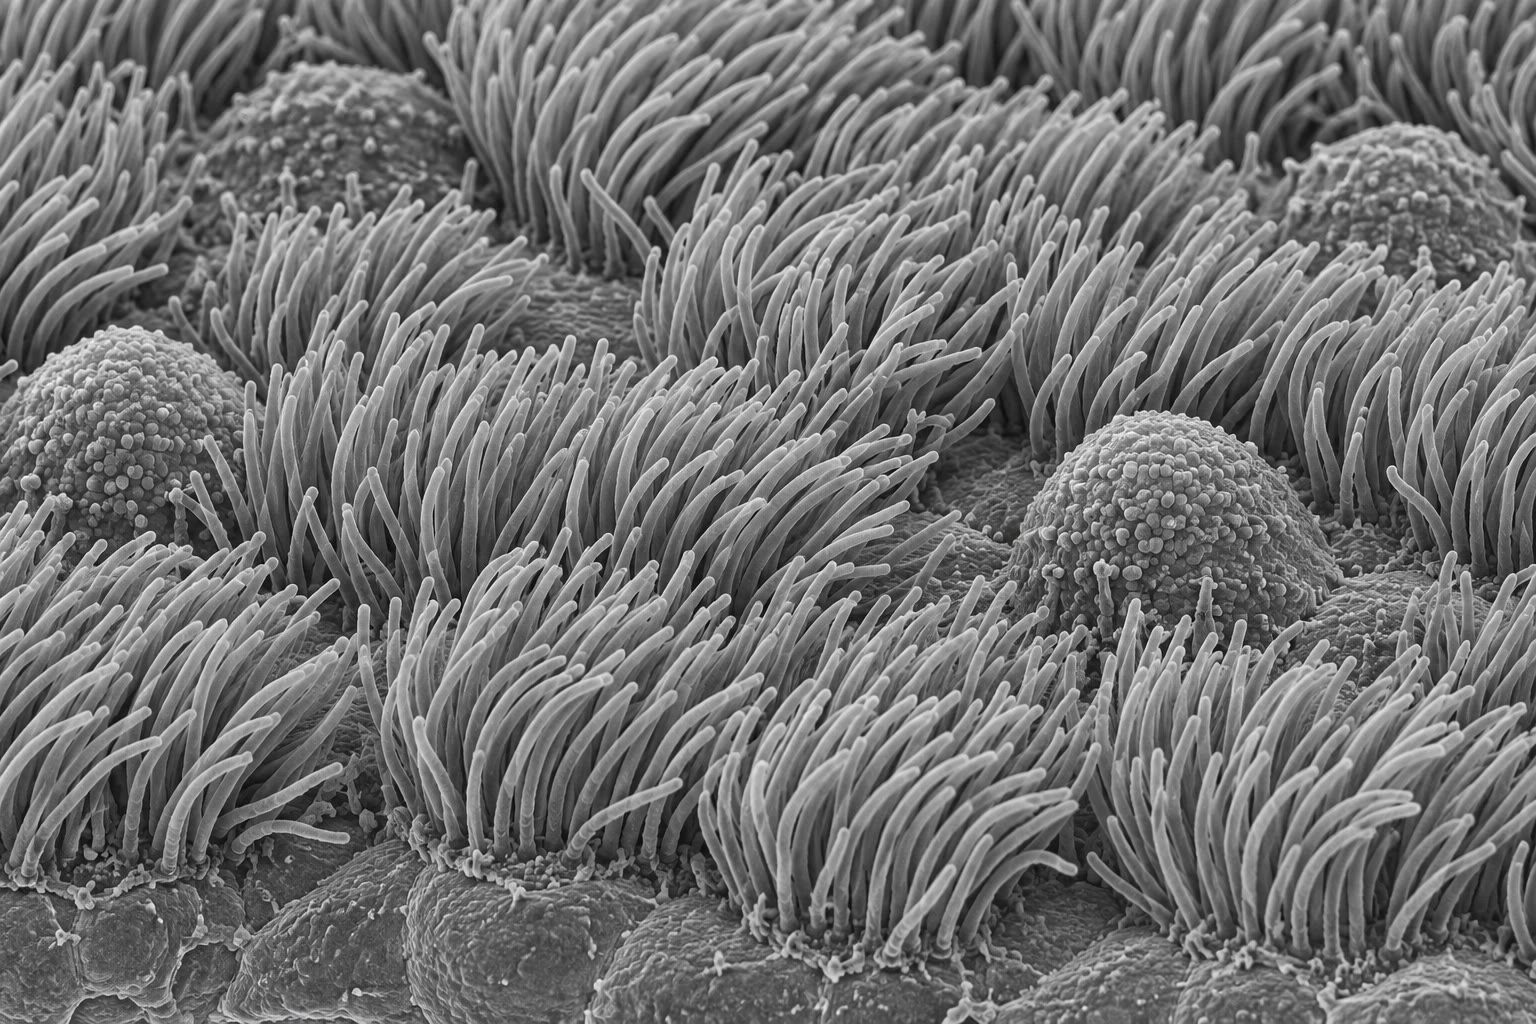
\includegraphics[width=0.54\linewidth]{images/book5/ai/b5-09-cilia-sem.jpg}\hspace{0.03\linewidth}
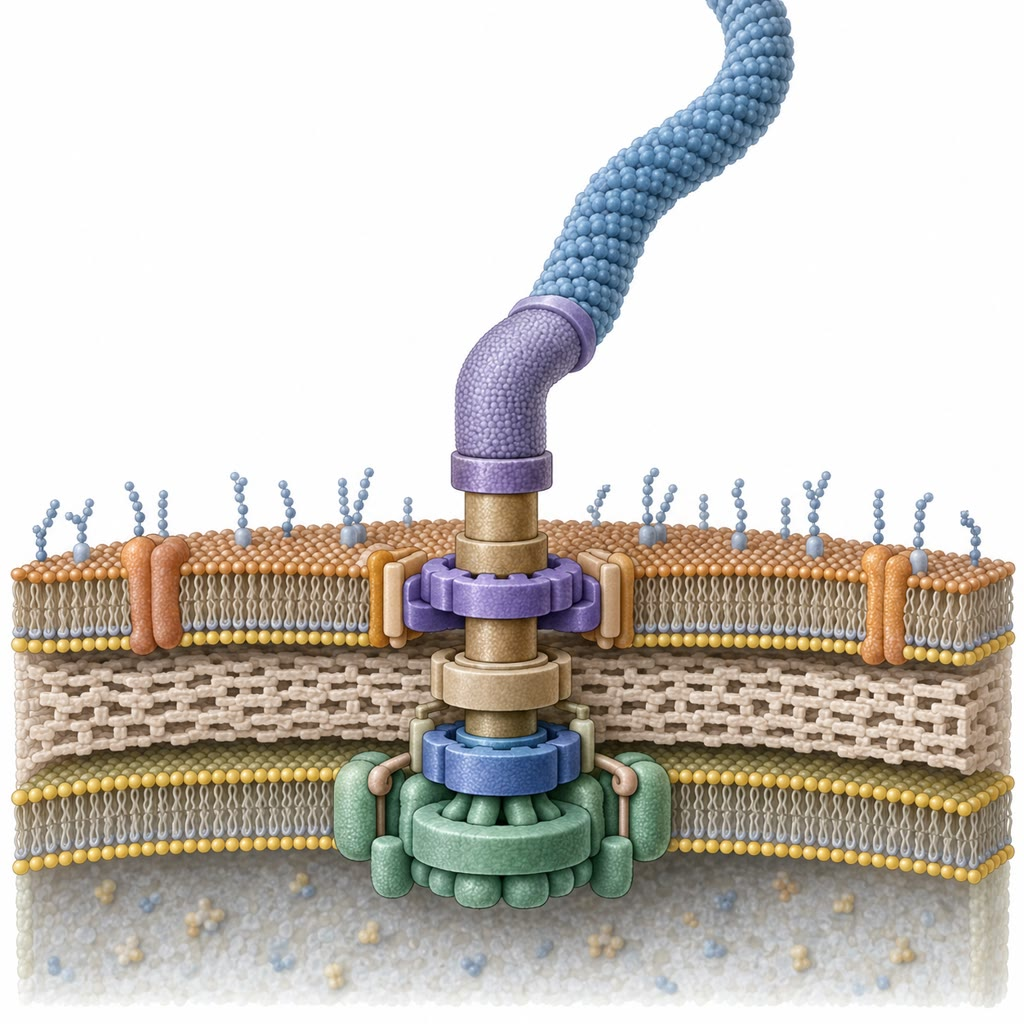
\includegraphics[width=0.36\linewidth]{images/book5/ai/b5-09-flagellar-motor.jpg}

{\small बाएँ: क्रमवीक्षी इलेक्ट्रॉन सूक्ष्मदर्शी में श्वासनली की
पक्ष्माभी उपकला, गुंबद-आकार की श्लेष्मा-स्रावी कोशिकाओं के बीच
\omterm{def:b3:cytoskeleton-motility:cilia}{पक्ष्माभों} की एक चादर। दाएँ: जीवाणु का \omterm{prop:b3:cytoskeleton-motility:flagellar-motor}{कशाभी मोटर}, कोशिका-आवरण में
वलयों का घूर्णी इंजन जो प्रोटॉनों के बहाव से चलता है।}
\end{omfigure}

\begin{proposition}[जीवाणु का कशाभी मोटर]\label{prop:b3:cytoskeleton-motility:flagellar-motor}
\index{कशाभी मोटर}\index{दौड़ और लुढ़कन}
जीवाणु का कशाभ सुकेंद्रकी कशाभ से असंबंधित है: फ़्लैजेलिन का कोई दृढ़
कुंडलित तंतु, \qty{20}{nm} मोटा और कई माइक्रोमीटर लंबा, जिसे
कोशिका-आवरण में जड़ा कोई \emph{घूर्णी मोटर} घुमाता है --- कोई पैंतालीस
प्रोटीनों का घूर्णक, जिसके चारों ओर स्थाणु इकाइयों का वलय है, और हर
इकाई ऐसी वाहिका है जिससे होकर प्रोटॉन अपनी प्रवणता के सहारे कोशिका में
बहते हैं, प्रति चक्कर लगभग एक हज़ार प्रोटॉन। मोटर \qty{300}{Hz} तक
घूमता है, एक मिलीसेकंड में दिशा उलट देता है, और कोई \qty{1000}{pN.nm}
बल-आघूर्ण बनाता है; वह लगभग बीस प्रोटीनों से बना है जिनके जीन उसी क्रम
में चालू होते हैं जिस क्रम में भाग जोड़े जाते हैं, भीतर से बाहर की ओर।
\emph{E.~coli} में वामावर्त घूर्णन कई कशाभों को किसी नोदक में बाँध देता
है और कोशिका सीधी \emph{दौड़ती} है; दक्षिणावर्त पर स्विच करते ही गुच्छा
बिखर जाता है और कोशिका किसी नई यादृच्छिक दिशा की ओर \emph{लुढ़क} जाती
है। रसायनानुचलन का पथ लुढ़कनों की बारंबारता के सिवा कुछ नहीं झुकाता
--- परिस्थितियाँ सुधरने पर कम --- और किसी प्रवणता पर चढ़ने के लिए इतना
ही पर्याप्त है।
\end{proposition}

\begin{remark}[कोशिका-कंकाल एक क्रिया है]\label{rem:b3:cytoskeleton-motility:verb}
इस अध्याय में बताई लगभग कोई भी चीज़ उस अर्थ में संरचना नहीं है जिसमें
कोई हड्डी है: \omterm{def:b3:cytoskeleton-motility:migration}{पर्णपाद} बहुलकन की एक लहर है,
\cref{ch:b3:cell-cycle-apoptosis} का तर्कु बढ़ती और ढहती
\omterm{def:b3:cytoskeleton-motility:filaments}{सूक्ष्मनलिकाओं} की एक स्थायी अवस्था, \omterm{def:b3:cytoskeleton-motility:cilia}{पक्ष्माभ} की ताल मोटरों का एक
स्विचिंग प्रतिरूप। आवागमन कोई लागत नहीं है जिसे कोशिका सह लेती है,
बल्कि वही क्रियाविधि है, इसीलिए इनमें से हर तंत्र न्यूक्लियोटाइड के
जल-अपघटन पर चलता है और ATP समाप्त होने के मिनटों में रुक जाता है, और
इसीलिए वे विष जो बहुलकों को किसी भी एक अवस्था में जमा देते हैं ---
टैक्सॉल या कोल्चिसीन, फैलॉयडिन या साइटोकैलेसिन --- समान रूप से घातक हैं।
\end{remark}

\section{अभ्यास}

\begin{exercise}[$\star$]\label{exo:b3:cytoskeleton-motility:1}
\omterm{def:b3:cytoskeleton-motility:filaments}{ऐक्टिन तंतुओं}, \omterm{def:b3:cytoskeleton-motility:filaments}{सूक्ष्मनलिकाओं} और \omterm{def:b3:cytoskeleton-motility:filaments}{मध्यवर्ती तंतुओं} की व्यास, उपइकाई,
ध्रुवता, न्यूक्लियोटाइड और प्रारूपिक भूमिका में तुलना कीजिए।
\end{exercise}

\begin{exercise}[$\star$]\label{exo:b3:cytoskeleton-motility:2}
\omterm{thm:b3:cytoskeleton-motility:treadmilling}{क्रांतिक सांद्रता} को परिभाषित कीजिए। किसी \omterm{def:b3:cytoskeleton-motility:filaments}{ऐक्टिन तंतु} के दोनों सिरों
की \omterm{thm:b3:cytoskeleton-motility:treadmilling}{क्रांतिक सांद्रताएँ} भिन्न क्यों होती हैं, और यदि वे बराबर होतीं तो
क्या होता?
\end{exercise}

\begin{exercise}[$\star$]\label{exo:b3:cytoskeleton-motility:3}
हर एक के लिए कोई मोटर बताइए: \omterm{def:b3:cytoskeleton-motility:filaments}{सूक्ष्मनलिकाओं} पर कोशिका-परिधि की ओर कोई
पुटिका; केंद्र की ओर कोई पुटिका; किसी प्रतिबल-तंतु का संकुचन; किसी
\omterm{def:b3:cytoskeleton-motility:cilia}{पक्ष्माभ} का मुड़ना। हर एक अपनी पटरी पर जो दिशा लेती है वह भी दीजिए।
\end{exercise}

\begin{exercise}[$\star$]\label{exo:b3:cytoskeleton-motility:4}
रेंगने के चक्र के चारों चरण और उनमें से पहले तीन को चलाने वाली
Rho-कुल की GTPase गिनाइए।
\end{exercise}

\begin{exercise}[$\star\star$]\label{exo:b3:cytoskeleton-motility:5}
किसी बहुलक के धन सिरे का $k_{\text{जुड़}} = \qty{5}{\micro M^{-1}.s^{-1}}$,
$k_{\text{छूट}} = \qty{1}{s^{-1}}$ है, और उसके ऋण सिरे का $k_{\text{जुड़}} =
\qty{1}{\micro M^{-1}.s^{-1}}$, $k_{\text{छूट}} = \qty{0.8}{s^{-1}}$।
दोनों \omterm{thm:b3:cytoskeleton-motility:treadmilling}{क्रांतिक सांद्रताएँ}, स्थायी-अवस्था सांद्रता और चक्रचालन दर
उपइकाई प्रति सेकंड में तथा, \qty{2.7}{nm} की उपइकाइयों के लिए,
नैनोमीटर प्रति सेकंड में ढूँढ़िए।
\end{exercise}

\begin{exercise}[$\star\star$]\label{exo:b3:cytoskeleton-motility:6}
\omterm{def:b3:cytoskeleton-motility:motors}{काइनेसिन} \qty{800}{nm/s} से \qty{8}{nm} के डग भरती है, हर डग पर एक ATP।
प्रति मोटर प्रति सेकंड कितने ATP? किसी न्यूरॉन का तंत्रिकाक्ष
\qty{1}{m} का है: यात्रा कितनी लंबी है, और एक मोटर उस पर कितने ATP खर्च
करती है? \cref{prop:b3:cytoskeleton-motility:physics} के विसरण-काल से तुलना कीजिए।
\end{exercise}

\begin{exercise}[$\star\star$]\label{exo:b3:cytoskeleton-motility:7}
\omterm{def:b3:cytoskeleton-motility:motors}{मायोसिन} V प्रति ATP \qty{36}{nm} का डग भरती है। उसका अधिकतम \omterm{prop:b3:cytoskeleton-motility:physics}{ठहराव बल}
क्या है, और वह \omterm{def:b3:cytoskeleton-motility:motors}{काइनेसिन} के बल से कम क्यों है? कौन-सी मोटर बड़ा भार ढोने
के लिए बेहतर है, और कौन-सी तेज़ चलने के लिए?
\end{exercise}

\begin{exercise}[$\star\star$]\label{exo:b3:cytoskeleton-motility:8}
किसी विभाजित होती कोशिका पर, और किसी रेंगती कोशिका पर, (क)
टैक्सॉल, (ख) कोल्चिसीन, (ग) साइटोकैलेसिन, (घ) किसी Rac निरोधक के
प्रभाव का पूर्वानुमान कीजिए, और हर एक को क्रियाविधि से समझाइए।
\end{exercise}

\begin{exercise}[$\star\star$]\label{exo:b3:cytoskeleton-motility:9}
किसी \omterm{def:b3:cytoskeleton-motility:migration}{पर्णपाद} पर किसी FRAP प्रयोग में प्रतिदीप्ति \qty{20}{s} के
अर्ध-काल के साथ अपने आरंभिक मान के \qty{90}{\%} तक लौट आती है। जाल में
ऐक्टिन का निवास-काल और अचल अंश क्या हैं?
चित्तियाँ \qty{1.5}{\micro m/min} से पीछे बहती हैं जबकि किनारा
\qty{1}{\micro m/min} से आगे बढ़ता है: किनारे पर ऐक्टिन किस दर से
बहुलकित हो रहा है?
\end{exercise}

\begin{exercise}[$\star\star\star$]\label{exo:b3:cytoskeleton-motility:10}
\omterm{def:b3:cytoskeleton-motility:instability}{गतिक अस्थिरता} को \omterm{def:b3:cytoskeleton-motility:instability}{GTP टोपी} के रूप में समझाइए, और दिखाइए कि \omterm{thm:b3:cytoskeleton-motility:treadmilling}{क्रांतिक
सांद्रता} से ठीक ऊपर रखी गई कोई \omterm{def:b3:cytoskeleton-motility:filaments}{सूक्ष्मनलिका} समष्टि लंबाई में एकसमान के
बजाय द्विबहुलकी क्यों हो जाती है। जो व्यवहार GTP बरबाद करता है उससे
कोशिका को क्या मिलता है?
\end{exercise}

\begin{exercise}[$\star\star\star$]\label{exo:b3:cytoskeleton-motility:11}
\qty{2}{\micro m} का कोई जीवाणु \qty{25}{\micro m/s} से तैरता है। इस
पैमाने पर पानी में श्यान कर्षण का बोलबाला है और मोटर के रुकते ही कोशिका
एक नैनोमीटर के भीतर रुक जाती है। समझाइए कि कोई प्रत्यागामी गति (कोई
चप्पू) उसे क्यों नहीं चला सकती और कोई घूमती कुंडली क्यों चला सकती है,
और \qty{100}{Hz} पर मोटर प्रति सेकंड कितने प्रोटॉन खर्च करता है, आँकिए।
\end{exercise}

\begin{exercise}[$\star\star\star$]\label{exo:b3:cytoskeleton-motility:12}
कार्टागेनर संलक्षण --- अचल \omterm{def:b3:cytoskeleton-motility:cilia}{पक्ष्माभ} --- जीर्ण श्वसनी-शोथ, पुरुष
बंध्यता, और आधे रोगियों में दाईं ओर हृदय देता है। हर एक को \omterm{def:b3:cytoskeleton-motility:cilia}{अक्षसूत्र} के
जीवविज्ञान से समझाइए, और बताइए कि अंतिम केवल आधों को क्यों प्रभावित
करता है।
\end{exercise}

\section{समस्या: चलता हुआ कोई उदासीनरागी}

\begin{problem}[{सप्तांत समस्या --- किसी उदासीनरागी का ऐक्टिन बजट गिना
गया, उसका चक्रचालन निकाला गया, किसी पुटिका की तंत्रिकाक्ष-यात्रा विसरण
के सामने समयबद्ध की गई, किसी मोटर की दक्षता मापी गई, और रेंगते भाग का
बहुलकन तथा ATP-लागत निकाली गई, जिसका अंत चक्रचालन दर, किसी तंत्रिकाक्ष
पार करने के समय और किसी पर्णपाद द्वारा प्रति सेकंड जलाए गए ATP पर होता
है}]
\label{pb:b3:cytoskeleton-motility:1}
आँकड़े: \qty{300}{\micro m^3} आयतन का कोई उदासीनरागी ऐक्टिन को
\qty{200}{\micro M} पर रखता है, जिसका आधा बहुलकित है; कोई उपइकाई किसी
तंतु में \qty{2.7}{nm} जोड़ती है। ऐक्टिन के दर-नियतांक
\cref{ex:b3:cytoskeleton-motility:actin-numbers} जैसे। \omterm{def:b3:cytoskeleton-motility:motors}{काइनेसिन}:
\qty{8}{nm} के डग, \qty{800}{nm/s}, \omterm{prop:b3:cytoskeleton-motility:physics}{ठहराव बल} \qty{6}{pN}; ATP जल-अपघटन
$\Delta G = \qty{50}{kJ/mol}$; $k_{B}T = \qty{4.1}{pN.nm}$; पुटिका का
विसरण गुणांक \qty{1}{\micro m^2/s}; तंत्रिकाक्ष की लंबाई \qty{1}{m}।
\omterm{def:b3:cytoskeleton-motility:migration}{पर्णपाद} \qty{20}{\micro m} चौड़ा है, प्रति माइक्रोमीटर किनारे पर $200$
तंतु हैं, और वह \qty{10}{\micro m/min} से आगे बढ़ रहा है; जाल किनारे से
\qty{3}{\micro m} पीछे टूट जाता है।

\medskip
\noindent\textbf{भाग I --- ऐक्टिन का बजट।}
\begin{enumerate}
  \item कोशिका में कितने ऐक्टिन अणु हैं, और कितने तंतुओं में हैं?
  \item वह कुल कितनी तंतु-लंबाई हुई? यदि औसत तंतु
        \qty{0.25}{\micro m} का हो तो कितने तंतु?
  \item मुक्त ऐक्टिन \qty{100}{\micro M} है, जो काँटेदार सिरे की
        \omterm{thm:b3:cytoskeleton-motility:treadmilling}{क्रांतिक सांद्रता} से बहुत ऊपर है। तंतु बस इतना क्यों नहीं
        बढ़ते कि एकलक समाप्त हो जाए? (दो प्रोटीन।)
  \item पात्रे चक्रचालन: दर-नियतांकों से $C_{\text{स्था}}$ और $J$
        निकालिए, और चक्रचालन की चाल नैनोमीटर प्रति सेकंड तथा
        माइक्रोमीटर प्रति मिनट में।
  \item कोशिका में प्रभावी चाल \qty{1}{\micro m/min} है। नियामक नंगे
        बहुलक को किस गुणक से तेज़ करते हैं?
  \item हर चक्रचालित उपइकाई पर एक ATP लगता है। यदि सारे $2\times 10^{5}$
        तंतु कोशिकीय चाल से चक्रचालन करें, तो प्रति सेकंड कितने ATP, और
        यह किसी कोशिका के प्रति सेकंड लगभग $10^{9}$ ATP के कुल आवागमन
        का कितना अंश है?
\end{enumerate}

\medskip
\noindent\textbf{भाग II --- तंत्रिकाक्ष से नीचे कोई पुटिका।}
\begin{enumerate}[resume]
  \item \omterm{def:b3:cytoskeleton-motility:motors}{काइनेसिन} से चलती कोई पुटिका तंत्रिकाक्ष पार करने में कितना समय
        लेती है, और मोटर कितने डग तथा ATP खर्च करती है?
  \item \qty{1}{m} पर विसरण को कितना समय लगता? किसी कोशिका-काय की
        चौड़ाई \qty{10}{\micro m} पर? इस तुलना से क्या निकलता है कि
        कोशिकाएँ विसरण पर कहाँ भरोसा कर सकती हैं?
  \item प्रति ATP ऊर्जा जूल में और $k_{B}T$ के मात्रकों में निकालिए।
  \item \qty{8}{nm} डग वाली किसी मोटर का अधिकतम बल, और ठहराव पर
        \omterm{def:b3:cytoskeleton-motility:motors}{काइनेसिन} की दक्षता।
  \item \qty{100}{nm} त्रिज्या की कोई पुटिका
        \qty{0.01}{Pa.s} श्यानता (पानी से दस गुना) वाले कोशिकाद्रव्य
        में \qty{800}{nm/s} से चलते हुए कर्षण $F = 6\pi\eta r v$ अनुभव
        करती है। उसे निकालिए, और \omterm{prop:b3:cytoskeleton-motility:physics}{ठहराव बल} से तुलना कीजिए: कितनी मोटर चाहिए?
  \item किसी न्यूरॉन का तंत्रिकाक्ष एक समय में लगभग $10^{4}$ पुटिकाएँ
        ढोता है। परिवहन की कुल ATP खपत प्रति सेकंड क्या है, और वह
        न्यूरॉन के प्रति सेकंड लगभग $10^{9}$ ATP के स्फुरण-व्यय से कैसी
        तुलना करती है? जिस न्यूरॉन की सूत्रकणिकाएँ विफल हो जाएँ, उसके
        लिए इसका क्या अर्थ है?
\end{enumerate}

\medskip
\noindent\textbf{भाग III --- अग्रभाग।}
\begin{enumerate}[resume]
  \item किनारे की चाल नैनोमीटर प्रति सेकंड में बदलिए, और निकालिए कि
        साथ बने रहने के लिए हर तंतु को प्रति सेकंड कितनी उपइकाइयाँ
        जोड़नी पड़ती हैं।
  \item कितने तंतु किनारे को धकेलते हैं, और पूरा किनारा प्रति सेकंड
        कितनी उपइकाइयाँ खपाता है?
  \item जुड़ी हर उपइकाई का अर्थ है एक ATP का जल-अपघटन, जो बाद में
        पुनर्चक्रित होता है। उभार के लिए प्रति सेकंड ATP; कोशिका के
        प्रति सेकंड $10^{9}$ का अंश।
  \item किनारे के पीछे का जाल \qty{3}{\micro m} गहरा है और वहीं टूटता
        है। जाल में किसी उपइकाई का जीवन-काल क्या है, और किसी भी समय
        जाल में कितनी उपइकाइयाँ हैं?
  \item झिल्ली उभार का विरोध प्रति तंतु लगभग \qty{1}{pN} के बल से
        करती है। जुड़ी प्रति उपइकाई किया गया काम
        ($F\times \qty{2.7}{nm}$) $k_{B}T$ में निकालिए और बताइए कि
        ब्राउनी रैचेट --- कोई तापीय उतार-चढ़ाव जो \qty{2.7}{nm} की झिरी
        खोल दे --- संभाव्य है या नहीं।
  \item लिस्टीरिया की धूमकेतु-पूँछ को कोई मोटर क्यों नहीं चाहिए, और यदि
        वह वही तंत्र बुला ले तो कितनी तेज़ी से धकेल सकती है?
\end{enumerate}

\medskip
\noindent\textbf{भाग IV --- दिशा।}
\begin{enumerate}[resume]
  \item उदासीनरागी किसी ऐसे रसायन-आकर्षक को भाँपता है जिसकी सांद्रता
        उसकी \qty{10}{\micro m} चौड़ाई पर \qty{2}{\%} बढ़ती है।
        \num{50000} ग्राहियों और माध्य सांद्रता के बराबर $K_{d}$ के
        साथ, आगे के आधे भाग पर पीछे के आधे भाग से कितने अधिक ग्राही
        अधिकृत हैं? (अधिकृति $\theta = C/(C +
        K_{d})$; प्रति ओर आधे ग्राही लीजिए।)
  \item किसी एक ओर अधिकृत संख्या में यादृच्छिक उतार-चढ़ाव लगभग उस संख्या
        का वर्गमूल है। क्या प्रश्न 19 का अंतर किसी एक क्षण में पकड़ में
        आता है? कुछ सेकंडों पर औसत लेने से क्या मदद मिलती है?
  \item कोशिका को स्रोत की ओर मुड़ने के लिए आगे कौन-सी GTPase और पीछे
        कौन-सी सक्रिय होनी चाहिए? हर जगह अनवरत सक्रिय Rac वाली कोशिका
        क्या करेगी?
  \item कोशिका \qty{30}{\micro m} दूर से \qty{3}{min} में जीवाणु तक
        पहुँच जाती है। आँकड़ों के सामने चाल की जाँच कीजिए।
  \item Arp2/3 से वंचित कोई कोशिका इसके बजाय बुलबुलन से --- दाब से
        चलने वाले झिल्ली के उभारों से --- चलती है। चक्र का कौन-सा चरण
        बदला गया है, और इससे दूसरे चरणों में ऐक्टिन की भूमिका के बारे
        में क्या पता चलता है?
  \item पूरा रेंगने का चक्र मिनट भर लेता है, फिर भी प्रवणता बदलते ही
        कोशिका सेकंडों में मुड़ जाती है। प्रश्न~16 के जाल के जीवन-काल
        से समझाइए।
  \item सारांश दीजिए: पात्रे चक्रचालन की चाल (प्रश्न~4), किसी पुटिका
        के तंत्रिकाक्ष पार करने का समय (प्रश्न~7), और उभार पर खर्च
        प्रति सेकंड ATP (प्रश्न~15)।
\end{enumerate}
\end{problem}
